\chapter{Estado del arte}

Las siguientes secciones describen algunos de las bases de datos más extendidas y usadas en la conducción autónoma, algunos modelos en redes neuronales exitosos en esta aplicación y algunos computadores especializados para el procesamiento de redes neuronales en tiempo real.

\section{Bases de datos para conducción autónoma}
\label{sec:datasets}

La tarea de la conducción autónoma requiere que el vehículo sea capaz de tomar decisiones en todo momento ante cualquier escenario posible en las vías por las que circula. Para ello hace uso de la información proporcionada por los sensores a bordo. El sensor más común y que más información aporta a la tarea de la conducción son las cámaras, que es la base de las redes que se explicarán en la siguiente sección. Para controlar todos los posibles escenarios en los que un vehículo puede verse involucrado hace falta un conjunto de datos lo suficientemente grande y representativo de todas ellas, y es por esto que en los últimos años y debido al auge de esta tecnología han aparecido multitud de bases de datos que ayudan a solucionar este problema.
    
\subsection{Comma.ai}

Comma.ai puso a disposición de la comunidad un conjunto de datos en 2016 \cite{comma} destinado a probar modelos de conducción autónoma basados en visión artificial. Este conjunto de datos cuenta con imágenes de vídeo obtenidas a partir de la conducción de una persona a bordo de un coche por entornos reales. En concreto, se dispone de 11 videoclips diferentes con un tamaño de fotograma de 160x320 píxeles, lo que hace un total de 45GB de datos, que se traducen en 7.25 horas de datos de conducción en entornos reales. Todos los fotogramas están etiquetados con información de: velocidad, aceleración, ángulo de giro, coordenadas GPS y ángulos del giroscopio a bordo del vehículo. Todos estos datos están registrados y sincronizados mediante marcas temporales, para que no haya desajuste entre los datos capturados por la cámara y la información de las etiquetas.

\subsection{Udacity}

Otro conjunto de datos popular para el problema de la conducción autónoma es el desarrollado por Udacity \cite{udacity-data}. De forma similar al conjunto de Comma.ai, este \textit{dataset} está formado por pequeños videoclips grabados bajo diferentes condiciones climatológicas: lluvia, sol, niebla.  Cuando nació este dataset constaba únicamente de 40GB de datos, lo que suponía un problema debido a la gran cantidad de información necesaria para entrenar modelos que solucionen el problema de la conducción autónoma en el mundo real. Por eso, se decidió ampliar este conjunto añadiendo más datos hasta los 223GB. En total recopila 70 minutos de conducción en entornos reales bajo diversas condiciones. Esta variación en la muestra se traduce en un mejor rendimiento de los modelos entrenados para la conducción autónoma, además de proporcionar información más realista de lo que un sistema que implemente una solución de este tipo se encontraría en el mundo real. Al igual que en el conjunto de Comma.ai, este conjunto de datos está etiquetado con información de velocidad, aceleración, ángulos de dirección, freno, marcha de la palanca de cambios, latitud y longitud.

\subsection {NuScenes}

Este mismo año se ha presentado una nueva base de datos multimodal a gran escala para la conducción autónoma denominada NuScenes \cite{nuscenes-dataset}. Esta base de datos se ha convertido en relevante al incluir información de toda una gama de sensores que incluye 5 radares, 1 lidar, 6 cámaras, IMU y GPS. NuTonomy scenes (NuScenes) tiene 7 veces más anotaciones y 100 veces más imágenes que el conjunto de datos de KITTI \cite{kitti-sim} que cubre 23 categorías incluyendo diferentes vehículos, tipos de peatones, dispositivos de movilidad y otros objetos.
Este conjunto de datos recopila 1000 escenas de conducción grabadas en Boston y Singapur, las cuales son ciudades conocidas por su gran densidad de tráfico y situaciones complejas en la conducción. Estas escenas duran 20 segundos y están seleccionadas manualmente para mostrar diversas y diferentes maniobras de conducción, situaciones en la circulación y comportamientos inesperados.
La mejora que aporta este conjunto de datos es que ofrece solución al desafío de que hay una falta de conjuntos de datos multimodales a gran escala. Esta multimodalidad es crítica, ya que ningún sensor es suficiente por sí solo y los tipos de sensores requieren cierta armonización, cosa de la que adolecen el resto de bases de datos mencionadas. En la Figura \ref{fig:nuscenes} se pueden ver algunos ejemplos de este conjunto de datos.

\begin{figure}
\begin{center}
	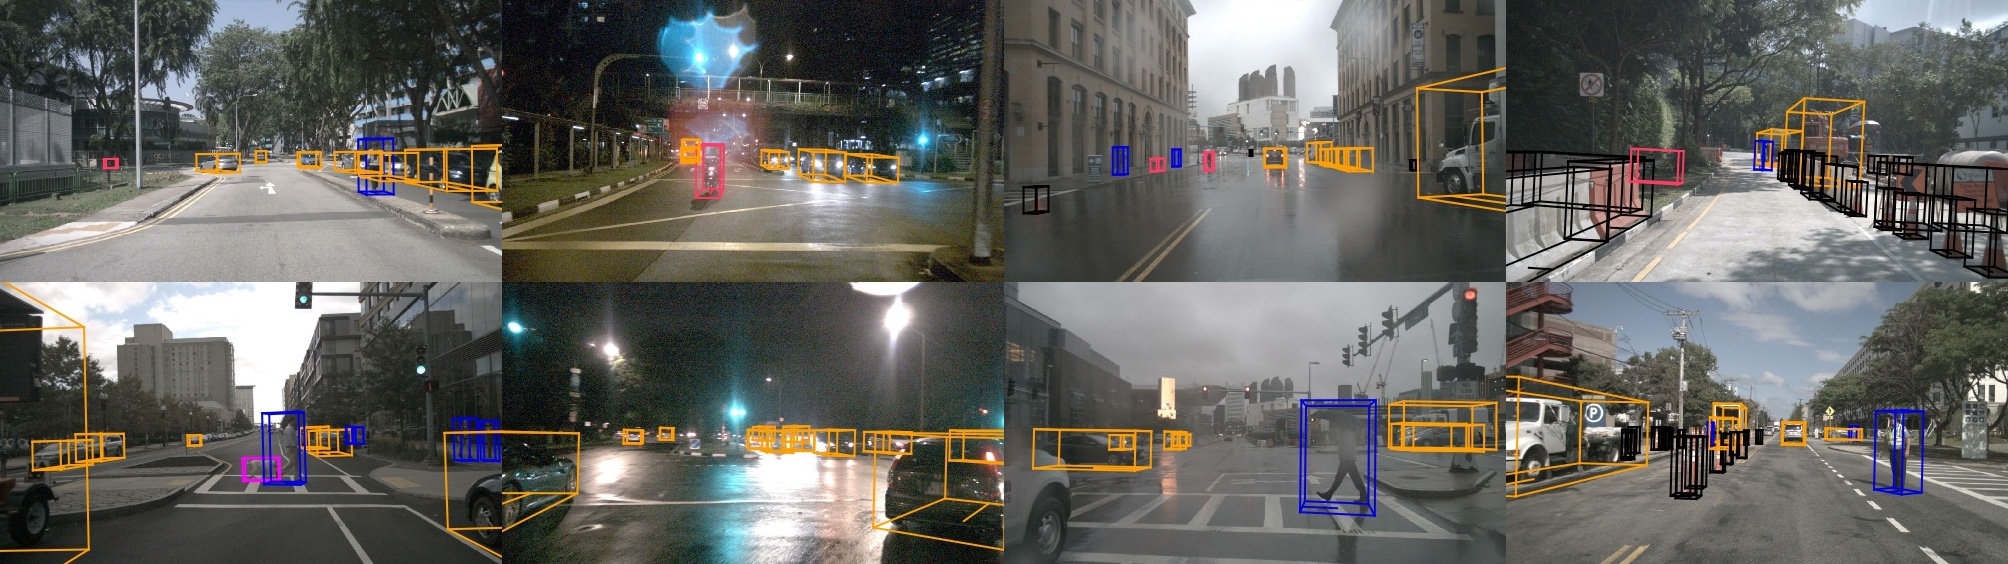
\includegraphics[width=0.8\textwidth]{img/nuscenes.jpg}
   \caption{Ejemplo de capturas del dataset NuScenes en diferentes situaciones climatológicas.}
	\label{fig.pilotnet}
\end{center}
\end{figure}

Además, se ha promovido el primer reto de detección de nuScenes que se lanzó en abril de 2019. Los ganadores y los resultados de los desafíos se anunciaron en el taller sobre conducción autónoma (\textit{nuScenes 3D detection challenge} como parte de \textit{the Workshop on Autonomous Driving at CVPR 2019}.).

\section{Redes neuronales para conducción autónoma}
\label{sec:nets}

Para cualquier comportamiento autónomo en robots es necesario un algoritmo que tome decisiones. En el caso de este proyecto, esos algoritmos están basados en redes neuronales y aprendizaje profundo, por lo que en esta sección se describirán algunas redes neuronales aplicadas al problema de conducción autónoma de forma exitosa en los últimos años en la comunidad investigadora.

\subsection{Redes neuronales convolucionales}

El problema de conducción autónoma no es novedoso, y el empleo de aprendizaje de extremo a extremo para solventar dicho problema tampoco, ya que se lleva explorando desde finales de los 80. El proyecto \textit{The Autonomous Land Vehicle in a Neural Network} (ALVINN) \cite{alvinn} fue desarrollado con el objetivo de atacar este problema desde la perspectiva de la visión artificial, al tratar de aprender ángulos de dirección a partir de la información sensorial proporcionada por un láser y un cámara, mediante una red neuronal con una sola capa oculta. Con el aprendizaje extremo a extremo como base, han surgido múltiples aproximaciones como \cite{road} \cite{end2end} \cite{interpretable}, que se detallan a continuación.

La red PilotNet \cite{end2end} \cite{explaining-end2end} es un ejemplo de red extremo a extremo. Esta red fue creada por NVIDIA y está descrita en el trabajo \cite{end2end}. Se trata de una red neuronal convolucional (CNN) que recibe una imagen frontal de la cámara del vehículo e infiere comandos de dirección. La medida de error se obtiene mediante la diferencia entre el comando inferido por la red neuronal y el comando deseado (supervisado) para una entrada en concreto, ajustando los pesos de la red en función de ese error mediante la técnica de \textit{back propagation}.

En la Figura \ref{fig.pilotnet} se ilustra la arquitectura de este tipo de red neuronal. Se puede observar que consta de 9 capas, divididas en 5 capas convolucionales, 3 capas densamente conexas y una capa extra de normalización. La imagen de entrada es preprocesada cambiando su espacio de color a YUV, que será la que alimente a la red tanto para entrenamiento como para inferencia. El diseño de esta red neuronal fue fruto de la experimentación en la que variaban las configuraciones de la diferentes capas. Las dos primeras capas convolucionales usan un \textit{stride} de 2x2 y un \textit{kernel} de 5x5, mientras que las tres últimas capas no usan \textit{stride} y su \textit{kernel} es de 3x3. El diseño de esta red consideraba que la capa densamente conexa fuera el controlador final de la dirección del robot, pero esto no es posible al no disponer de control sobre qué capas de la red funcionan como extractores de características y qué capas funcionan como controladoras. Como en toda red neuronal convolucional, las características se van aprendiendo en el entrenamiento del modelo de forma automática.

El principal objetivo de \cite{explaining-end2end} es tratar de explicar cómo aprende PilotNet y cómo la red realiza su toma de decisiones. Para ello, NVIDIA desarrolla un método para determinar los elementos de la imagen que más peso tienen en la decisión final de la red. Existe un informe detallado de dicho método en \cite{visual}.

\begin{figure}
\begin{center}
	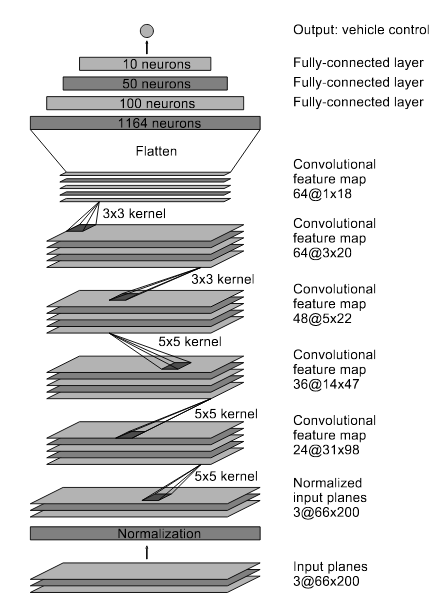
\includegraphics[width=0.3\textwidth]{img/pilotnet.png}
   \caption{Arquitectura Pilotnet.}
	\label{fig.pilotnet}
\end{center}
\end{figure}

Definen objeto saliente como los elementos de la imagen que más influyen en la toma de decisiones de la red, por lo tanto, para encontrar dichos objetos, se centran en localizar las partes de la imagen donde los mapas de características tienen mejores activaciones. En \cite{explaining-end2end} se explica todo el procedimiento y proponen un algoritmo para este fin, que se basa en hacer que las activaciones de los mapas de nivel superior se conviertan en máscaras para las activaciones de niveles inferiores. La Figura \ref{fig.salient} muestra ejemplos de objetos salientes para tres imágenes de entrada. Se pueden observar las regiones de la imagen que contribuyen más a la salida de la red.

\begin{figure}
\begin{center}
	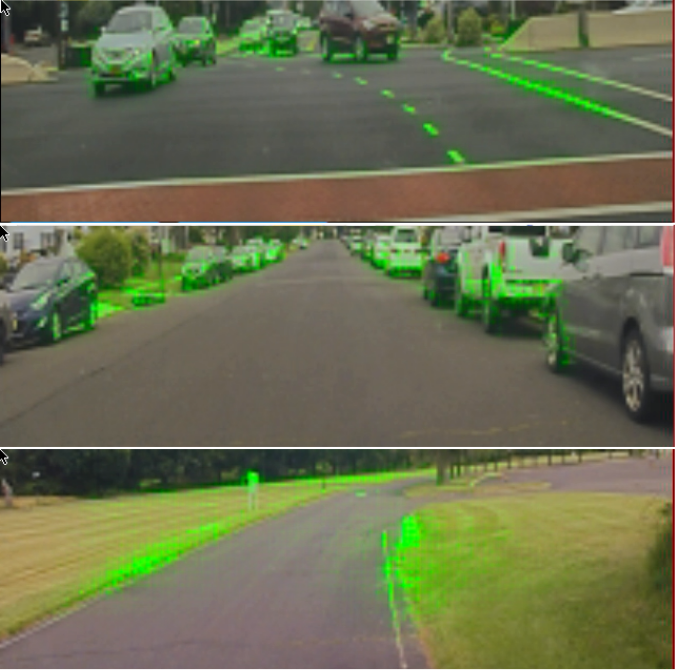
\includegraphics[width=0.4\textwidth]{img/saliencia.png}
   \caption{Ejemplos de objetos salientes para varias imágenes de entrada.}
	\label{fig.salient}
\end{center}
\end{figure}

Todas estas técnicas hacen que PilotNet aprenda a reconocer objetos que aportan información útil de la carretera mejorando su toma de decisiones y haciendo que la red sea capaz de realizar una conducción autónoma segura manteniendo el coche en el carril bajo multitud de situaciones, tanto si las líneas que demarcan el carril están presentes como si no.

Derivada de la red explicada anteriormente (PilotNet), surge una nueva arquitectura denominada TinyPilotNet propuesta en \cite{self-driving}. Esta nueva red, que se puede observar en la Figura \ref{fig.tinypilotnet}, está compuesta por 6 capas dispuestas como sigue: la capa de entrada que se alimenta de imágenes de resolución 16x32 píxeles con un único canal de color en espacio HSV, las siguientes dos capas son dos capas convolucionales configuradas con un \textit{kernel} de 3x3 y una capa de \textit{dropout} al 50\% de probabilidad; la salida de estas capas produce un tensor que se convierte en un vector que alimentará las dos últimas capas densamente conexas con cabezal clasificador biclase, para predecir los valores de dirección y aceleración.

En \cite{event} se propone un método para predecir el ángulo de giro de los vehículos: emulación de cámaras de eventos. Las cámaras de eventos son sensores que obtienen información de píxel de forma asíncrona a través de cambios en intensidad de la luz. Estos eventos se transforman en fotogramas mediante acumulación de píxeles en un intervalo constante de tiempo, lo que genera una imagen únicamente de eventos en 2D en un intervalo dado, que serán procesadas por una red neuronal profunda para asignar los ángulos de dirección. Las redes empleadas para el procesamiento de estas imágenes son redes con arquitectura residual, las ResNet; en concreto las redes ResNet18 y ResNet50. Se utilizan principalmente como extractores de características en problemas de regresión teniendo en cuenta únicamente las capas convolucionales. La codificación de las características obtenidas en la última capa convolucional en forma de vector, se lleva a cabo mediante una capa de \textit{global average pooling} que retorna la media del canal de las características extraídas, para posteriormente agregar una capa densamente conexa, con activación ReLu y otra capa densamente conexa unidimensional para inferir el ángulo.

\begin{figure}
\begin{center}
	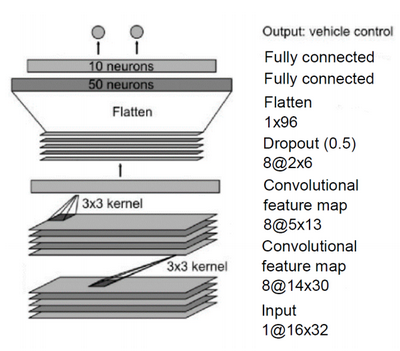
\includegraphics[width=0.5\textwidth]{img/tinypilotnet.png}
   \caption{Arquitectura TinyPilotnet.}
	\label{fig.tinypilotnet}
\end{center}
\end{figure}

\noindent En \cite{event} se infieren los ángulos emplenado tres tipos de entradas:

\begin{itemize}
    \item Imágenes en escala de grises
    \item Diferencia de imágenes en escala de grises
    \item Imágenes creadas por acumulación de eventos.
\end{itemize}

Se analiza el rendimiento de los modelos midiendo el tiempo de integración empleado para la generación de imágenes de eventos. A mayor cantidad de tiempo, mayor cantidad de eventos se capturan en los contornos de los objetos. Empíricamente se ha comprobado que un lapso de tiempo de $ 50 ms $ para la generación de la imágenes de eventos, el rendimiento de la red mejora, ya que tiempos más grandes degradan el rendimiento de la red al obtenerse imágenes más grandes. Como desventaja, si se emplean imágenes en escala de grises, a altas velocidades las imágenes se difuminan y se vuelven muy ruidosas.

En el trabajo \cite{pixels} se lleva a cabo un estudio donde se analiza el rendimiento de una red neuronal extremo a extremo para la conducción autónoma en base a las imágenes capturadas por el vehículo. Además se realiza un estudio comparativo entre las redes de clasificación y regresión, y el impacto que tienen las dependencias temporales de imágenes consecutivas. Parten de una variación de las arquitecturas PilotNet, VGG o Alexnet realizando modificaciones sobre ellas. Uno de los estudios de este trabajo es el impacto del grado de granularidad del número de clases de salida en el rendimiento del sistema. Además se evalúan los métodos que permiten la inclusión de la temporalidad en las imágenes: qué impacto tiene la inclusión de entradas consecutivas en el sistema a través del empleo de arquitecturas extremo a extremo con capas recurrentes.

El método \textit{stacked frames} consiste en el apilado de imágenes temporalmente consecutivas para la creación de una imagen apilada. Sea $I_t$ un fotograma en el instante $t$, este método apila además los fotogramas $I_{t-1}$, $I_{t-2}, etc.$ que servirán como entrada a la red. El formato de los vectores resultantes de este apilado crece en en la dimensión del canal (en profundidad), así, una imagen $I_T$ con dimensiones $224x224x3$ con las imágenes $I_{t-1}$ e $I_{t-2}$ apiladas, tendría unas dimensiones de $224x224x9$. Con la aplicación de este método se demuestra que el rendimiento de la red mejora. La conclusión obtenida es que esta mejora puede deberse a que la red puede tomar una decisión basada en la información promedio de múltiples fotogramas apilados. Si se utiliza una sola imagen, se carece de información contextual de lo que el vehículo ha percibido anteriormente, por lo que las predicciones pueden variar en gran medida. Sin embargo, con éste método, la información contextual puede servir para contener predicciones extremas al poder cancelarse la información entre sí. No obstante, esto tiene un límite, ya que apilar demasiadas imágenes puede provocar que la red pierda poder de generalización deteriorando su rendiminto; por ello se apilan únicamente tres fotogramas.

\subsection{Redes neuronales recurrentes}

Las redes neuronales recurrentes (RNN) presentan una técnica novedosa en cuanto al modelado de las relaciones temporales de los datos de entrada. Para ello emplean lo que denominan células de memoria. No obstante estas células de memoria están limitadas a relaciones temporales de corto alcance, por lo que con la inclusión de las \textit{Long Short-Term Memory} más comúnmente denominadas LSTM, que modelan relaciones temporales de largo alcance, se solventa este inconveniente.

Estas redes son especialmente útiles cuando los datos tienen el componente de la temporalidad, es decir se trata de secuencias de datos relacionadas en el tiempo. En múltiples estudios se ha hecho uso de la capacidad de estas redes para aprovechar la información secuencial para investigaciones sobre conducción autónoma.

En \cite{reactive-ground} se emplean este tipo de arquitecturas recurrentes, más concretamente las LSTM. Fruto de este estudio, se obtiene un controlador reactivo basado en aprendizaje profundo mediante una arquitectura de red neuronal muy sencilla que requiere pocas imágenes para realizar un entrenamiento efectivo. Esta arquitectura es bautizada como ControlNet, y supera a otras redes más complejas tanto en su aplicación en entornos interiores y exteriores haciendo uso de diferentes plataformas robóticas. Esta red se alimenta de imágenes en color (RGB) para realizar inferencia sobre ellas y obtener comandos de control. La arquitectura de esta red, que se puede observar en la Figura \ref{fig.controlnet}, implementa capas convolucionales (para extraer información sobre características de las imágenes de entrada) con sus capas de \textit{pooling} y capas densamente conexas (que actúan como clasificadores) alternas. Además, como se ha explicado, implementa una capa LSTM que incorpora información temporal, permitiendo que el vehículo pueda continuar con la misma dirección sobre fotogramas consecutivos similares.

\begin{figure}
    \makebox[\textwidth][c]{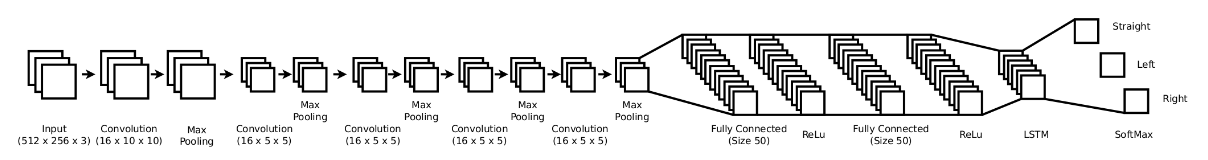
\includegraphics[width=1.3\textwidth]{img/controlnet.png}}%
    \caption{Estructura de red ControlNet.}
	\label{fig.controlnet}

\end{figure}

En \cite{temporal-dependencies} se crea la denominada \textit{Convolutional Long Short-Term Memory Recurrent Neural Network}, más conocida conocido como C-LSTM que se muestra en la Figura \ref{fig.clstm}. Este tipo de red neuronal se entrena extremo a extremo con el objetivo de que aprenda las dependencias temporales y visuales involucradas en la tarea de la conducción autónoma. Este sistema está compuesto de dos tipos de redes: las CNN y las LSTM y se alimenta de las imágenes capturadas por la cámara a bordo del vehículo para realizar inferencia del ángulo de giro en base a la información sensorial. Las características de la imagen se obtienen a través de la CNN fotograma a fotograma para aprender las dependencias visuales. Estas características son entonces procesadas por la LSTM para aprender las dependencias temporales. Al final de esta arquitectura existe un cabezal clasificador que predice el ángulo de giro del vehículo. En este sistema se aplica el concepto de \textit{transfer learning}, cuya idea fundamental se basa en realizar un entrenamiento adicional sobre una red pre-entrenada sobre un dominio concreto totalmente distinto del que fue entrenado. En este caso, la CNN está pre-entrenada en el conjunto de datos de Imagenet \cite{imagenet}, que es un conjunto de datos de 1,000,000 imágenes anotadas de objetos cotidianos agrupados en 1,000 clases diferentes. Los pesos entrenados de esa CNN sobre ImageNet son transferidos a otra red de dominio específico para imágenes de conducción, donde se reentrena partiendo de los pesos ya aprendidos en el primer entrenamiento. Posteriormente, la LSTM aprende las dependencias temporales de los vectores de características obtenidos por la CNN para tomar una decisión. 

\begin{figure}
\begin{center}
	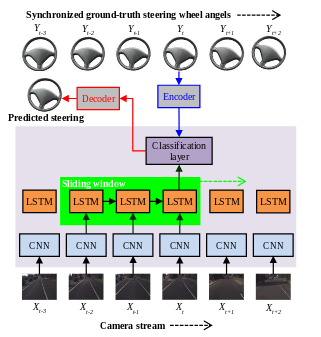
\includegraphics[width=0.5\textwidth]{img/clstm.png}
   \caption{Arquitectura C-LSTM.}
	\label{fig.clstm}
\end{center}
\end{figure}

Un trabajo similar se propone en \cite{deep-steering}. En este caso se propone un modelo de \textit{deep learning} que a partir de imágenes captadas por una cámara a bordo del vehiculo, se infieren ángulos de dirección dividiéndolo en dos subredes: una subred extractora de características y otra subred de predicción de dirección.

La subred extractora de características genera un vector de longitud fija (128 características) que modela la información sensorial y el estado del vehículo. Para esto, emplea una capa denominada \textit{spatio-temporal convolution} o ST-Conv y otra capa LSTM denominada ConvLSTM que modifican las dimensiones espacio-temporales de las imágenes de entrada. Posteriormente, se emplea una capa densamente conexa para obtener el vector de 128 características mencionado. Este vector alimenta a la siguiente subred de predicción de dirección.

La subred de dirección trata de concatenar la información de 3 fuentes: el vector de la subred extractora de características, la información del estado del vehículo y las acciones de dirección posibles. Para esto se incluye un paso de recurrencia entre la capa de salida y antes y después de las capas <<concatenadoras>> llamadas \textit{concat}. Se tiene que:

\begin{itemize}
    \item La capa \textit{concat} que precede a la capa LSTM agrega 3 características más al vector de 128 inicial: la velocidad, el ángulo de la rueda y el par de torsión.
    \item La capa \textit{concat} que va después de la capa LSTM está compuesta de un vector de características por un vector de 195 características: 128 de la primera subred + 64 de la LSTM + 3 de la capa \textit{concat} anterior.
\end{itemize}

Por su parte, en \cite{interpretable} se propone un trabajo similar a los anteriores al introducir un modelo de atención visual para el entrenamiento extremo a extremo de una red neuronal convolucional. El modelo de atención tiene en cuenta las zonas de la imagen que más afectan a la inferencia potencialmente. Este modelo predice órdenes de dirección a través de píxeles crudos, teniendo como salida el radio de giro inverso $\hat{u}_t$, que se relaciona con el ángulo de dirección utilizando la geometría de Ackermann.

Este modelo en concreto, al igual que los anteriores, se ayuda de las CNN para la extracción de un vector de características codificadas, a las que llaman características convolucionales cubo $x_t$, a partir de las imágenes de entrada captadas por la cámara del vehículo. Cada uno de esos vectores de características puede contener información descriptiva de los objetos de la imagen (a alto nivel) que permite una atención selectiva de diferentes zonas de la imagen. Para llevar a cabo este trabajo, hacen uso de la red PilotNet (explicada al principio de esta sección) para conseguir un modelo de conducción. La particularidad de este modelo es que la información espacial de la imagen es muy importante, por lo que omiten las capas de \textit{pooling} de la red para evitar la pérdida de esa información. Con esto, se genera un cubo $x_t$ tridimensional de características que pasa a través de las capas LSTM que estiman el $\hat{u}_t$ (radio de giro inverso). Como elemento final de este método se incluye un decodificador que es alimentado con un mapa de atención visual y ofrece como salida las detecciones de saliencias visuales locales.


\section{\textit{Hardware} acelerador de cómputo neuronal}

Hasta ahora se han visto dos elementos esenciales del problema de la conducción autónoma mediante redes neuronales: las propias redes neuronales y los conjuntos de datos con los que se entrenan. Debido al carácter de los datos a procesar, donde se tiene información sensorial proveniente de cámaras (de color, de profundidad, de lineales, etc.) que ofrece una enorme cantidad de datos en cada imagen captada, es indispensable una alto poder computacional para procesar todos esos datos de forma eficiente y en tiempo real.

La conducción autónoma es una tarea en la cual el tiempo real es un aspecto crítico, ya que se trata un problema cuya solución ha abordarse desde una perspectiva de control híbrida (planificación + reacción) donde se requiere que la toma de decisiones por parte del algoritmo sea muy rápida para poder reaccionar de forma instantánea ante la gran cantidad de escenarios imprevistos que se pueden suceder durante la conducción (peatones que cruzan sin mirar, accidentes de tráfico, animales que cruzan la vía, etc.). No obstante, no todos los vehículos pueden estar dotados de computadores de grandes dimensiones como podría ser un computador de escritorio debido a las limitaciones tanto de alimentación como de espacio. Por este motivo, algunas empresas como Google o NVIDIA han creado \textit{hardware específico} para solventar este problema y ya no solo para aplicarlo a la conducción autónoma, sino también a cualquier problema domótico o, como tecnología en auge, IoT (\textit{Internet of Things}). 

En esta sección se describirán diferentes dispositivos diseñados para ser suficientemente potentes al ejecutar una red neuronal pesada y ocupar el mínimo espacio físico posible con el objetivo de empotrarlo en algún sistema.

\subsection{NVIDIA Jetson TK1}

En 2014, NVIDIA presentaba su primera placa para sistemas embebidos de alto rendimiento y bajo consumo, denominada Jetson TK1 \cite{jetsontk1}. Esta placa de dimensiones muy reducidas (127mm x 127mm) cuenta con un procesador ARM de 32-bits con 2 núcleos y una GPU con arquitectura Kepler que implementa 192 núcleos CUDA, ambos incluidos en el SoC (\textit{System-on-Chip}) Tegra K1 \cite{tegrak1}, además de una memoria RAM de 2 GB con tecnología DDR3. La presentación del procesador Tegra K1 fue un todo un hito, ya que fue el primer procesador móvil que igualaba en rendimiento a sistemas de escritorio con un bajísimo consumo de energía de $12.5\ W$ a máxima carga. 

\begin{figure}[htp]
    \centering
    \captionsetup{justification=centering}
    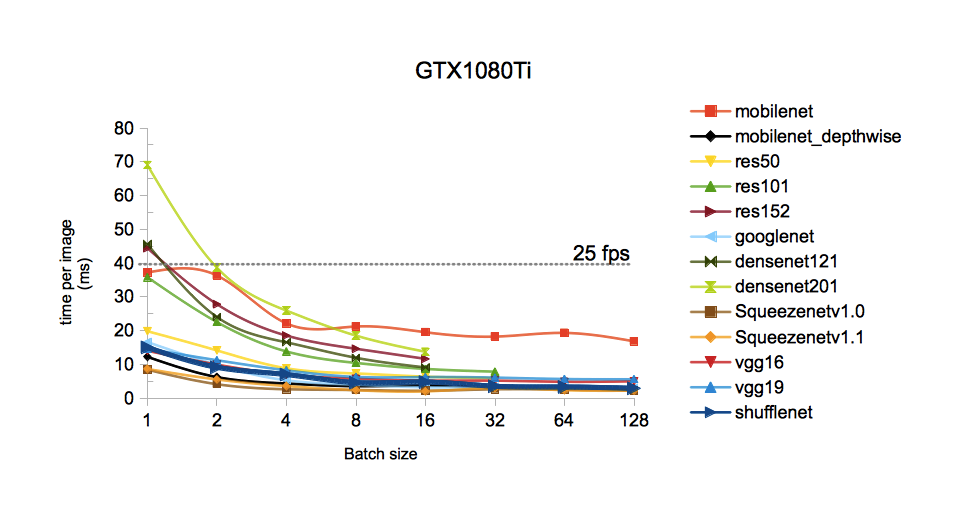
\includegraphics[width=.5\textwidth]{img/gtx1080_linear.png}\hfill
    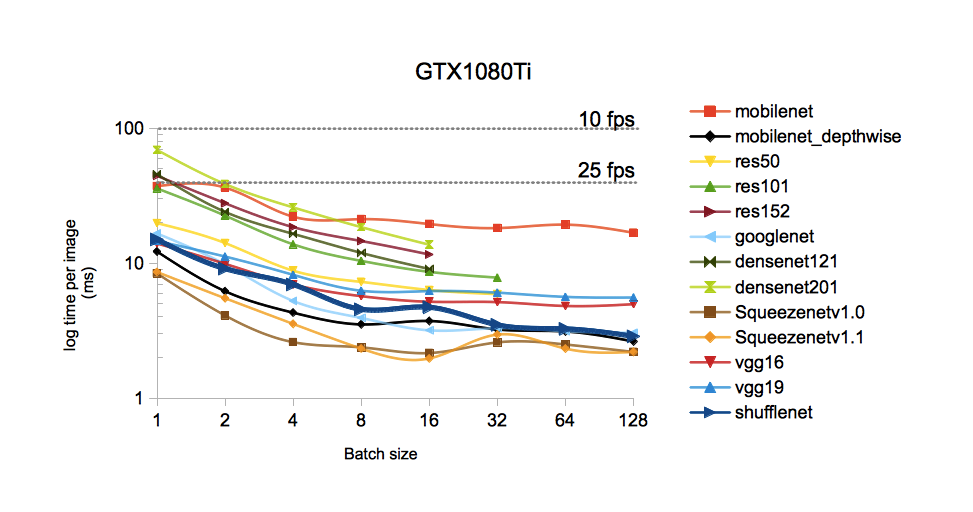
\includegraphics[width=.5\textwidth]{img/gtx1080_log.png}
    \caption{Banco de pruebas de referencia de la NVIDIA GTX 1080 de escritorio. (Izquierda) tiempo de procesamiento lineal. (Derecha) tiempo de procesamiento en escala logarítmica.}
    \label{fig:ben_gtx}
\end{figure}

\begin{figure}[htp]
    \centering
    \captionsetup{justification=centering}
    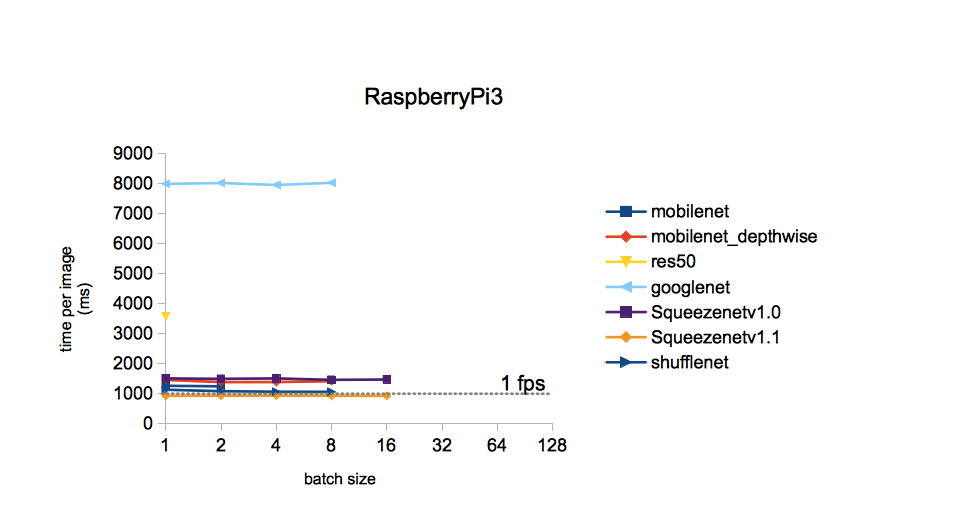
\includegraphics[width=.5\textwidth]{img/Raspi_linear.png}\hfill
    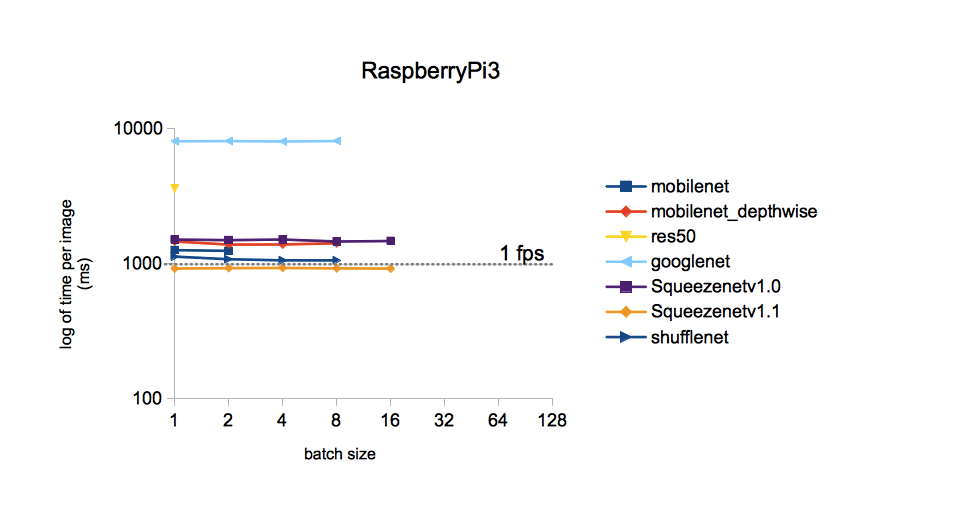
\includegraphics[width=.5\textwidth]{img/Raspi_log.png}
    \caption{Banco de pruebas de referencia de una Raspberry Pi3. (Izquierda) tiempo de procesamiento lineal. (Derecha) tiempo de procesamiento en escala logarítmica.}
    \label{fig:ben_pi}
\end{figure}

Se han realizado algunos bancos de pruebas de esta placa probando su rendimiento con la ejecución de algunas redes neuronales modernas desarrolladas para sistemas embebidos, como \textit{mobilenet}, \textit{googlenet} o \textit{shufflenet} entre otras. Como referencia, en la Figura \ref{fig:ben_gtx} se tiene este mismo banco de pruebas medido sobre una tarjeta gráfica de alta gama para sistemas de escritorio, la NVIDIA GTX 1080Ti como referencia techo, y en la Figura \ref{fig:ben_pi} la referencia suelo de este mismo banco de pruebas llevado a una RaspberryPi modelo 3.

Los resultados se miden como la media de tiempo (en $ms$) que tarda el SoC TK1 en procesar una imagen frente a un tamaño de lote determinado de la red neuronal. Como se puede observar en la Figura \ref{fig:ben_tk1} (izquierda), la red más lenta es la \textit{mobilenet} con un tiempo de procesamiento por imagen de casi medio segundo ($500\ ms$), mientras que la red más rápida es la \textit{shufflenet v1.1} con un tiempo de procesamiento por debajo de los $100\ ms$, lo que aporta una tasa de fotogramas por segundo relevante. En la Figura \ref{fig:ben_tk1} (derecha) se puede apreciar con mayor claridad el rendimiento de esta placa con diferentes redes neuronales.

No obstante, si se compara esta placa con una RaspberryPi 3, los resultados son significativos, ya que su rendimiento es más del doble con respecto a la Raspberry. Y si se compara por arriba con la GTX 1080, no está muy lejos de los mínimos de esta, por lo que el poder computacional con respecto a la energía consumida es notable. Todo esto se puede ver reflejado en la Figura \ref{fig:ben_tk1_comp}

\begin{figure}[htp]
    \centering
    \captionsetup{justification=centering}
    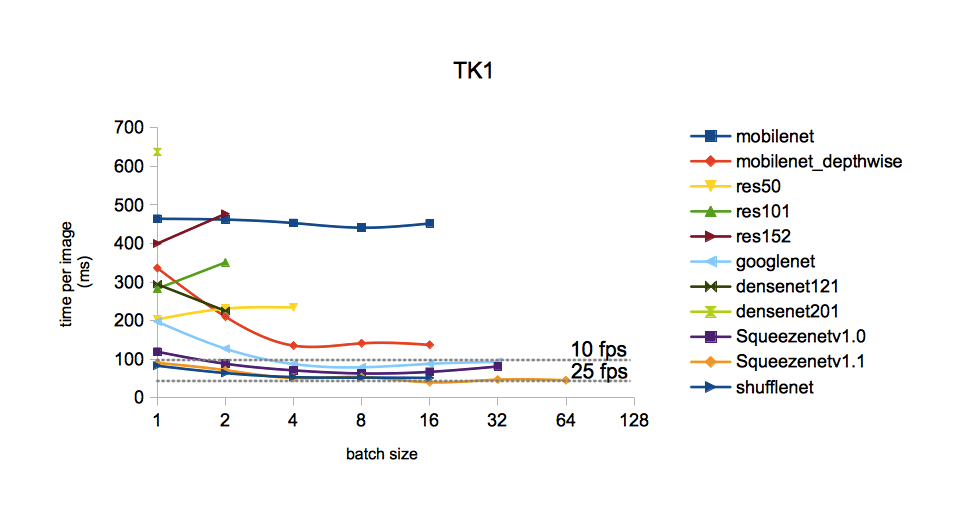
\includegraphics[width=.5\textwidth]{img/TK1_linear.png}\hfill
    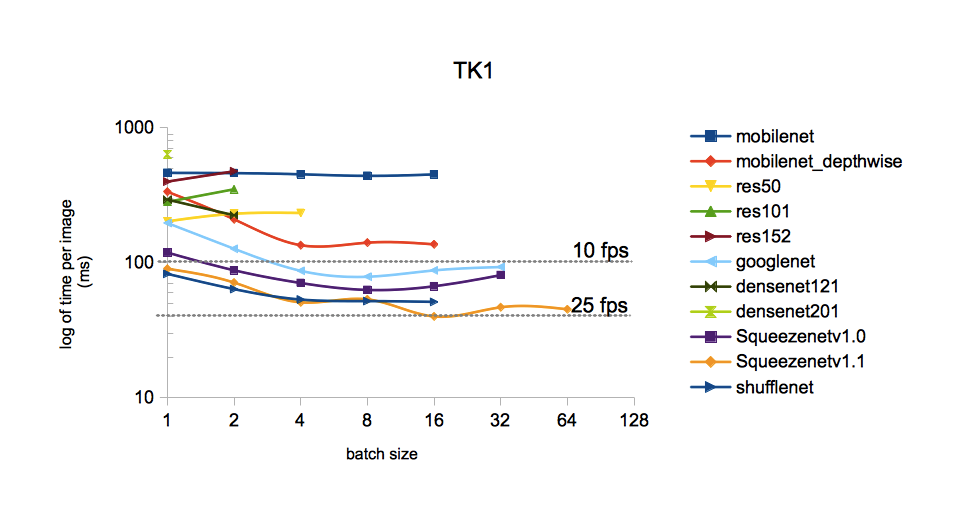
\includegraphics[width=.5\textwidth]{img/TK1_log.png}
    \caption{banco de pruebas para la NVIDIA Jetson TK1. (Izquierda) tiempo de procesamiento lineal. (Derecha) tiempo de procesamiento en escala logarítmica.}
    \label{fig:ben_tk1}
\end{figure}

\begin{figure}[htp]
    \centering
    \captionsetup{justification=centering}
    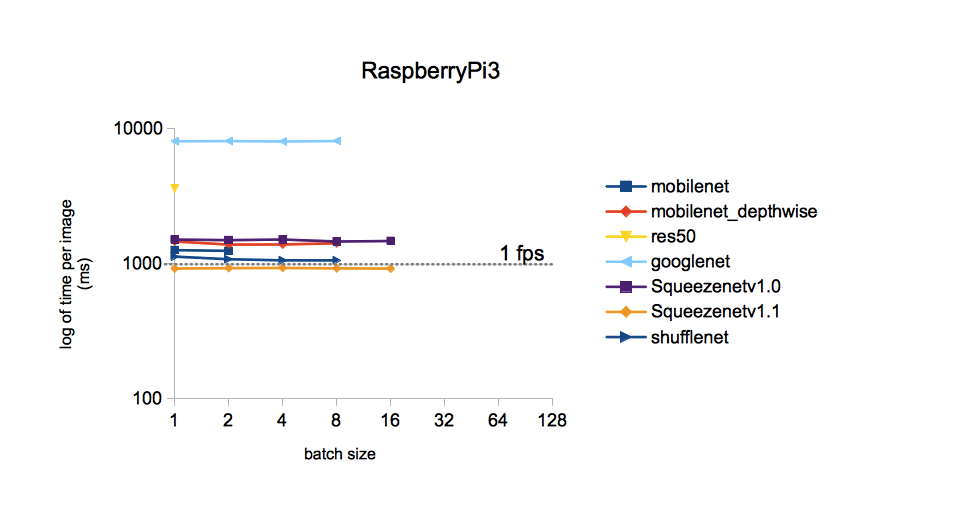
\includegraphics[width=.33\textwidth]{img/Raspi_log.png}\hfill
    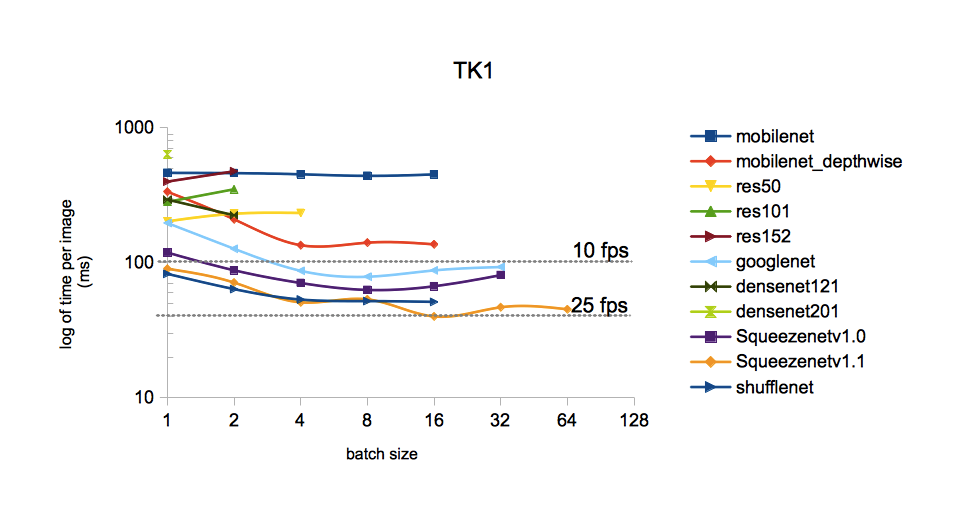
\includegraphics[width=.33\textwidth]{img/TK1_log.png}\hfill
    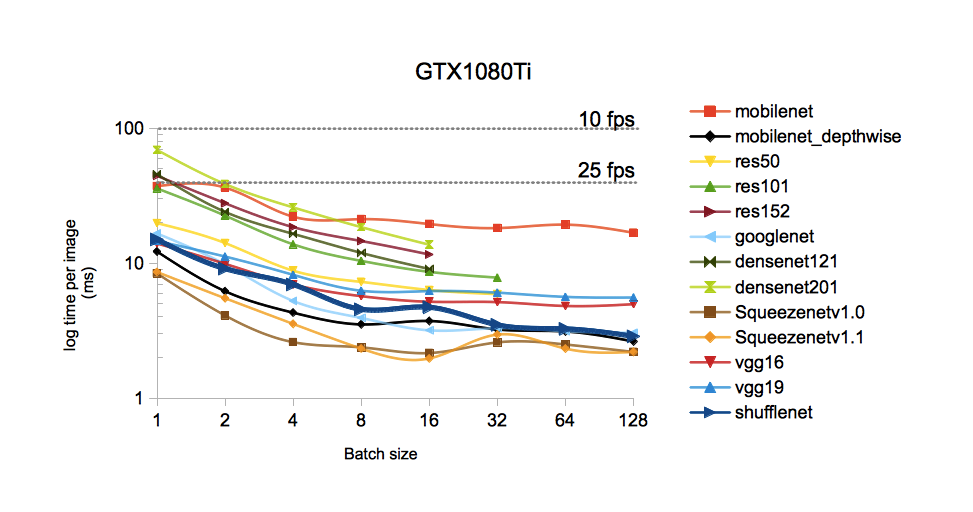
\includegraphics[width=.33\textwidth]{img/gtx1080_log.png}
    \caption{Comparativa entre RaspberryPi 3 (izquierda), Jetson TK1 (centro) y GTX 1080Ti (derecha).}
    \label{fig:ben_tk1_comp}
\end{figure}

\subsection{NVIDIA Jetson TX1}

En 2015, NVIDIA dio un paso adelante con su nueva placa para sistemas empotrados: la Jetson TX1 \cite{jetsontx1}. Esta placa de dimensiones aún más reducidas que su predecesora (50mm x 87mm) cuenta con un procesador ARM de 64-bits con 4 núcleos y una GPU con arquitectura Maxwell, ambos incluídos en el SoC (\textit{System-on-Chip}) Tegra X1, además de una memoria RAM de 4 GB con tecnología LPDDR4. Este módulo supuso un salto en capacidad de cómputo ya que el procesador dobla en poder al de la Jetson TK1 tanto en CPU como en GPU. Este salto en potencia también se ve reflejado en el consumo, ya que a máxima carga, esta placa consume 15 W frente a los 12.5 W de la TK1.

En la Figura \ref{fig:ben_tx1} se reflejan los resultados de los bancos de pruebas aplicados a esta placa. Comparando con los resultados de la placa TK1 (Figura \ref{fig:ben_tk1}), a simple vista se puede percibir que el salto en rendimiento y potencia es evidente. Mientras que la Jetson TK1, no es capaz de ofrecer tasas de refresco mayores que 25 fotogramas por segundo, la Jetson TX1 supera ese umbral en más de la mitad de las redes probadas. Y las redes más lentas como la \textit{densenet201} obtienen una mejora de rendimiento significativa en la placa TX1.
Comparada con la GTX 1080Ti (Figura \ref{fig:ben_gtx}), se puede ver que el rendimiento de la TX1 se acerca mucho a los resultados obtenidos por la 1080Ti. Hay que tener en cuenta que la placa Jetson TX1 cuenta con una tecnología propietaria de NVIDIA denominada Maxwell, cuyo chip implementa 256 núcleos CUDA; mientras que la GTX 1080Ti cuenta con una tecnología más avanzada, también propietaria de NVIDIA, denominada Pascal y cuyo chip implementa 3584 núcleos CUDA.

\begin{figure}[htp]
    \centering
    \captionsetup{justification=centering}
    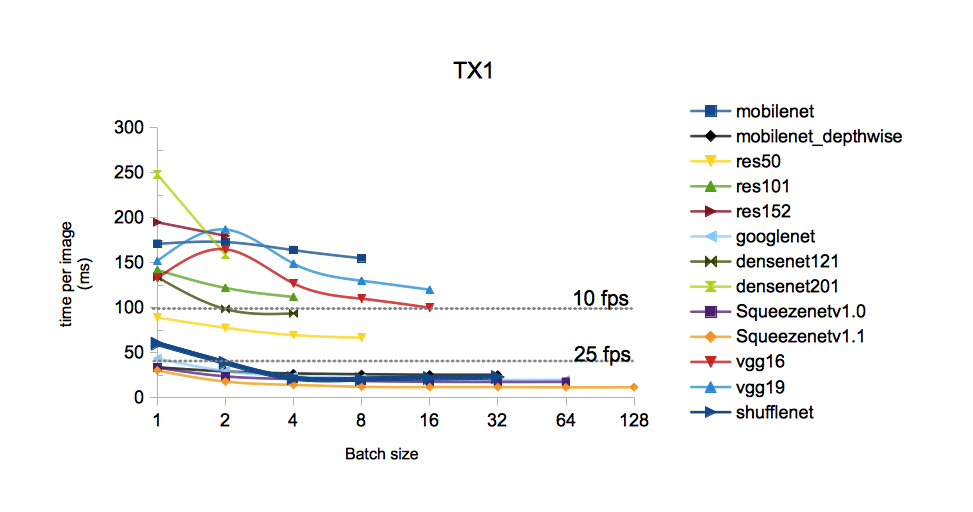
\includegraphics[width=.5\textwidth]{img/TX1_linear.png}\hfill
    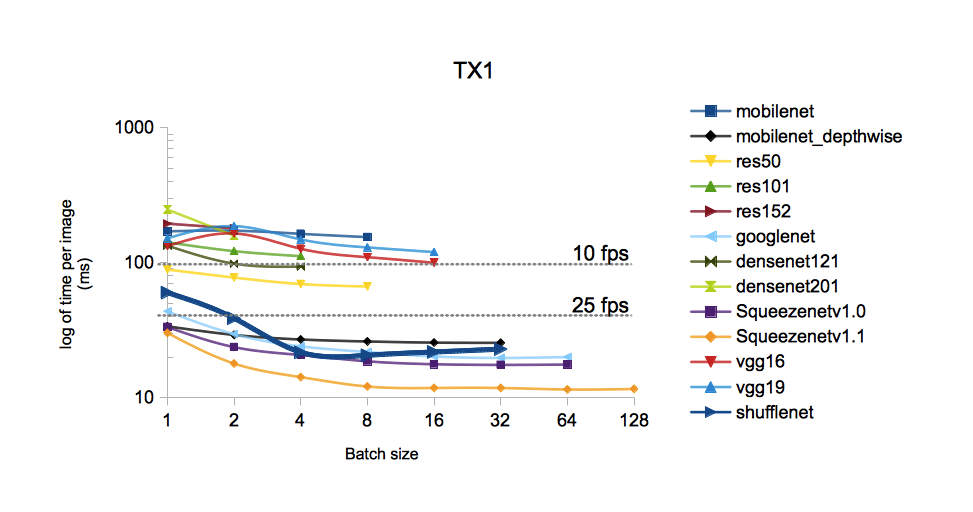
\includegraphics[width=.5\textwidth]{img/TX1_log.png}
    \caption{banco de pruebas para la NVIDIA Jetson TX1. (Izquierda) tiempo de procesamiento lineal. (Derecha) tiempo de procesamiento en escala logarítmica.}
    \label{fig:ben_tx1}
\end{figure}

\begin{figure}[htp]
    \centering
    \captionsetup{justification=centering}
    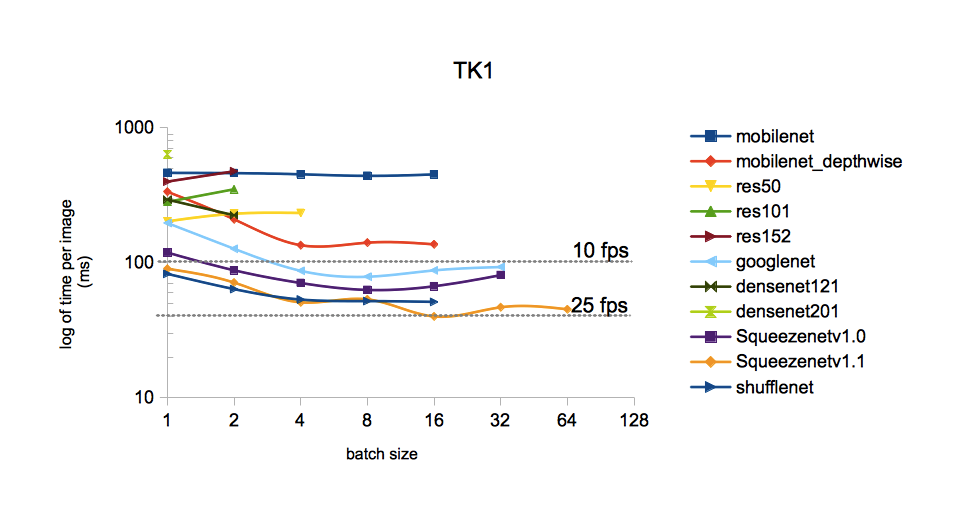
\includegraphics[width=.33\textwidth]{img/TK1_log.png}\hfill
    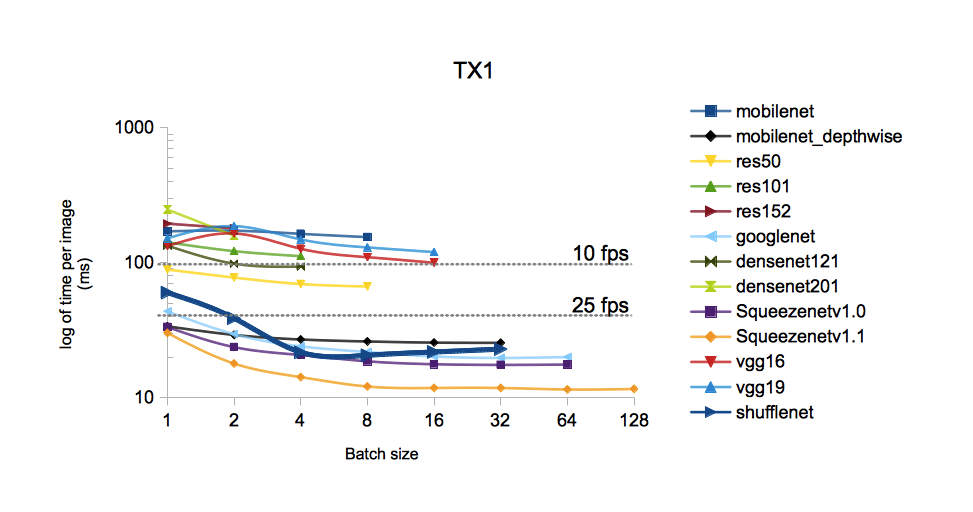
\includegraphics[width=.33\textwidth]{img/TX1_log.png}\hfill
    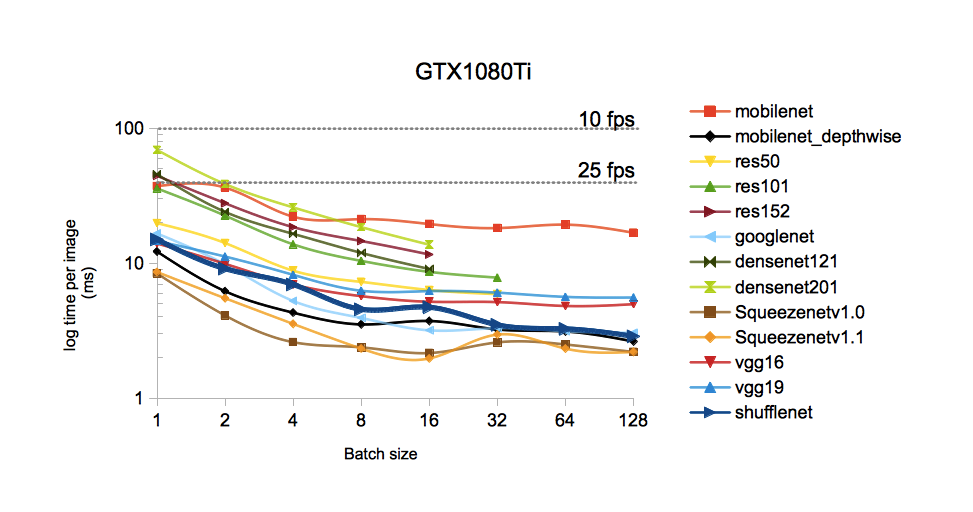
\includegraphics[width=.33\textwidth]{img/gtx1080_log.png}
    \caption{Comparativa entre Jetson TK1 (izquierda), Jetson TX1 (centro) y GTX 1080Ti (derecha). Escala logarítmica.}
    \label{fig:ben_tk1_comp_1080}
\end{figure}

\subsection{NVIDIA Jetson Nano}
\label{sec:jnano}

En 2019 NVIDIA presentó sus nuevas placas de precio y prestaciones reducidas denominadas Jetson Nano \cite{jetsonnano}. Estas nueva placas siguen la línea de sus hermanas con un tamaño reducido (80mm x 100mm) pero con precio y prestaciones más bajos, aunque muy potentes y optimizadas para inteligencia artificial. Cuenta con un procesador ARM de 64-bits con 4 núcleos y una GPU basada en tecnología Maxwell (como sus hermana Jetson TX1) con la mitad de núcleos CUDA (128). Este módulo tiene dos modos de consumo: modo normal (5W) y carga máxima (10W), lo que lo hace el más liviano de toda la gama Jetson, además tiene un precio reducido con respecto al resto de placas de la familia. Cabe destacar que el modo de consumo normal desactiva parte del hardware de la placa, ya que apaga 2 núcleos del procesador para ahorrar energía. No obstante, a máxima potencia, ofrece el máximo rendimiento hardware.

En la Figura \ref{fig:ben_nano} se tiene el resultado de los tests en la Jetson Nano. Comparado con su hermana la Jetson TX1 (Figura \ref{fig:ben_tx1}) se puede apreciar que el rendimiento es ligeramente más bajo debido a que tiene la mitad de núcleos en su CPU y su frecuencia de trabajo es más baja. No obstante, si se compara con la Jetson TK1 (Figura \ref{fig:ben_nano_comp} (izquierda)), se puede comprobar que la supera en rendimiento en todas las redes probadas. Hay que tener en cuenta, en este caso concreto, el consumo de ambas placas y el número de núcleos de GPU de ambas. Mientras que la Jetson TK1 cuenta con 192 núcleos CUDA en su GPU, la Jetson Nano cuenta con 128 núcleos. Además, el consumo de la Jetson TK1 es más del doble que la Jetson Nano. Con todo eso, esta placa es superior a la TK1 en cuanto a ratio rendimiento/consumo. Para la misma red \textit{mobilenet}, la placa Nano bate en rendimiento a la TK1 acercándose a una tasa de fotogramas por segundo de 10, mientras que la TK1 permanece constante muy alejada de esos valores.

\begin{figure}[htp]
    \centering
    \captionsetup{justification=centering}
    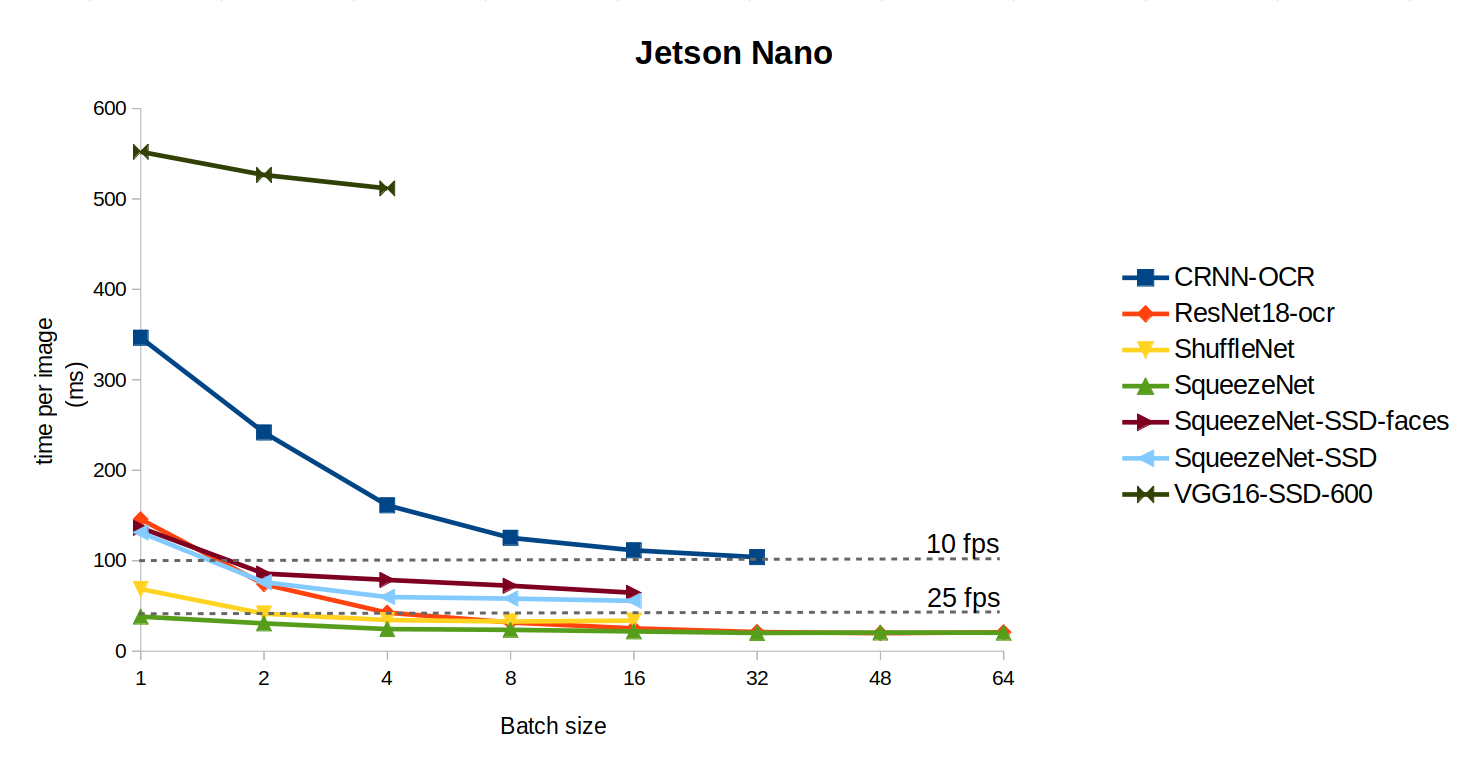
\includegraphics[width=.5\textwidth]{img/Jetson-nano-linear.png}\hfill
    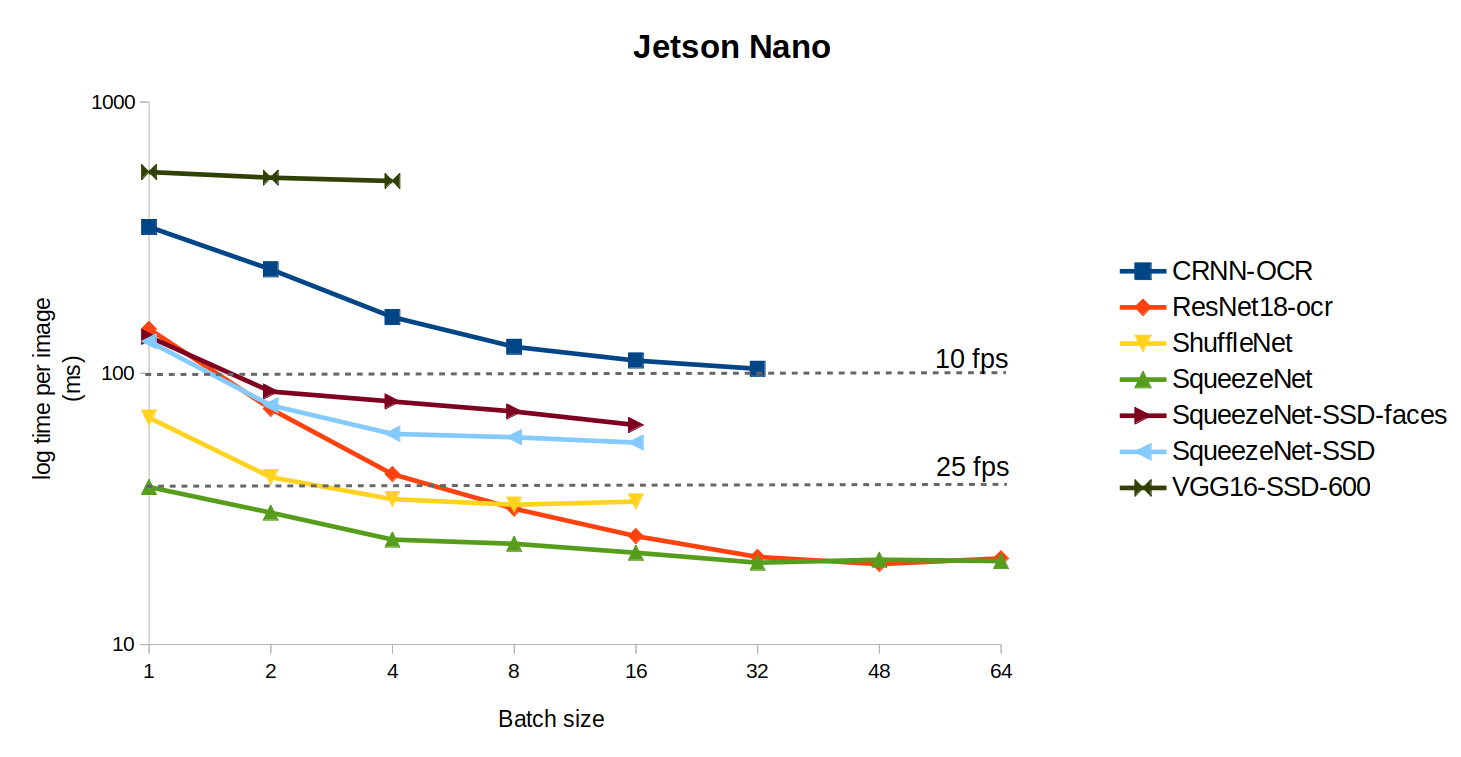
\includegraphics[width=.5\textwidth]{img/Jetson-nano-log.png}
    \caption{banco de pruebas para la NVIDIA Jetson Nano. (Izquierda) tiempo de procesamiento lineal. (Derecha) tiempo de procesamiento en escala logarítmica.}
    \label{fig:ben_nano}
\end{figure}

\begin{figure}[htp]
    \centering
    \captionsetup{justification=centering}
    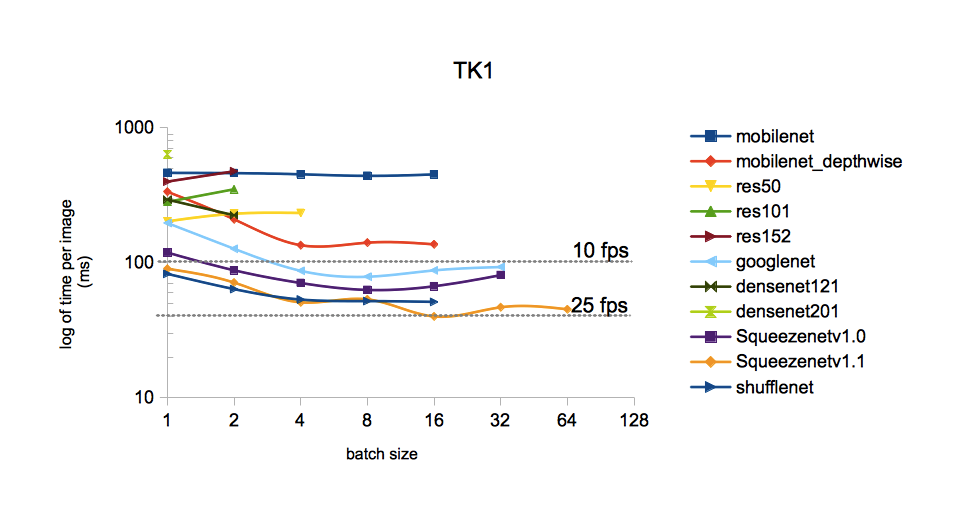
\includegraphics[width=.33\textwidth]{img/TK1_log.png}\hfill
    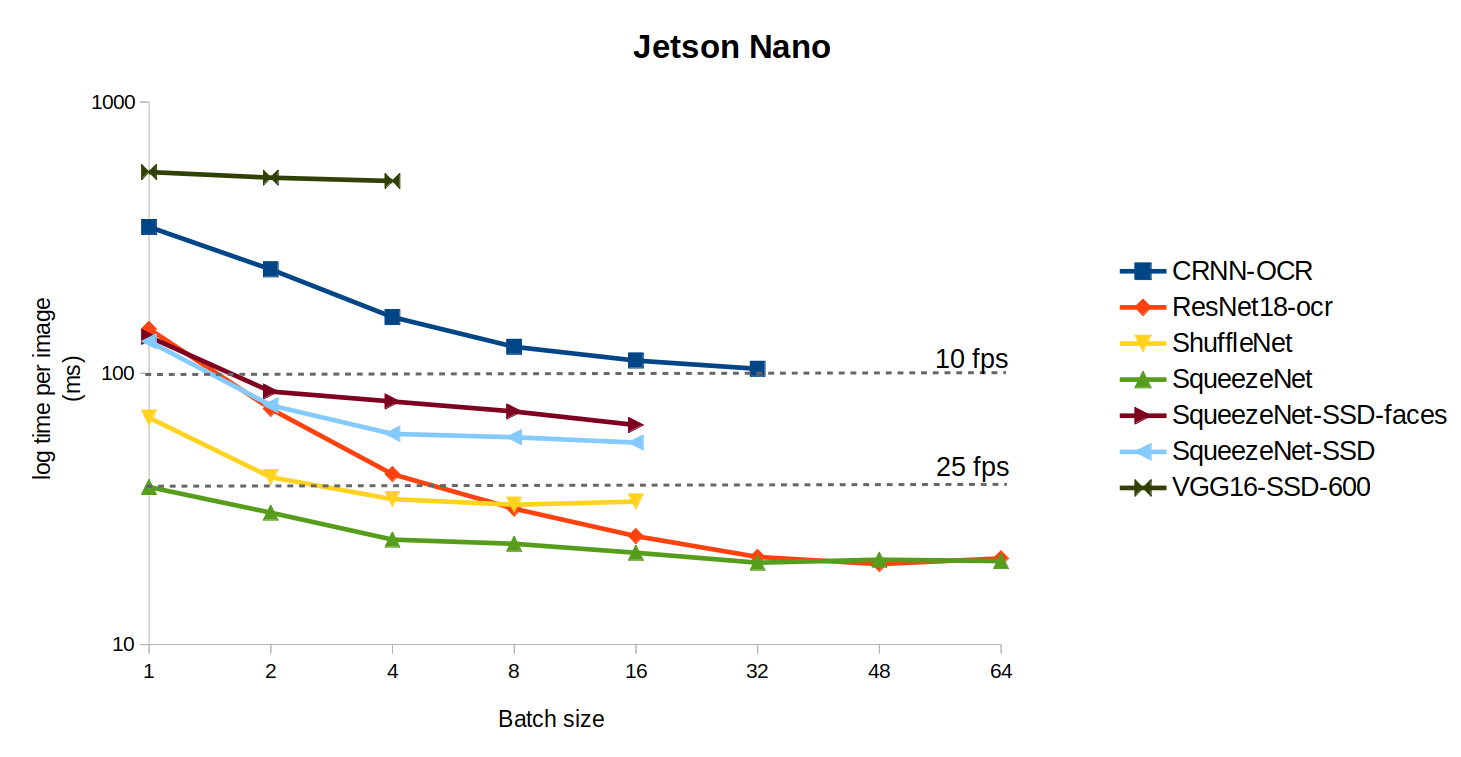
\includegraphics[width=.33\textwidth]{img/Jetson-nano-log.png}\hfill
    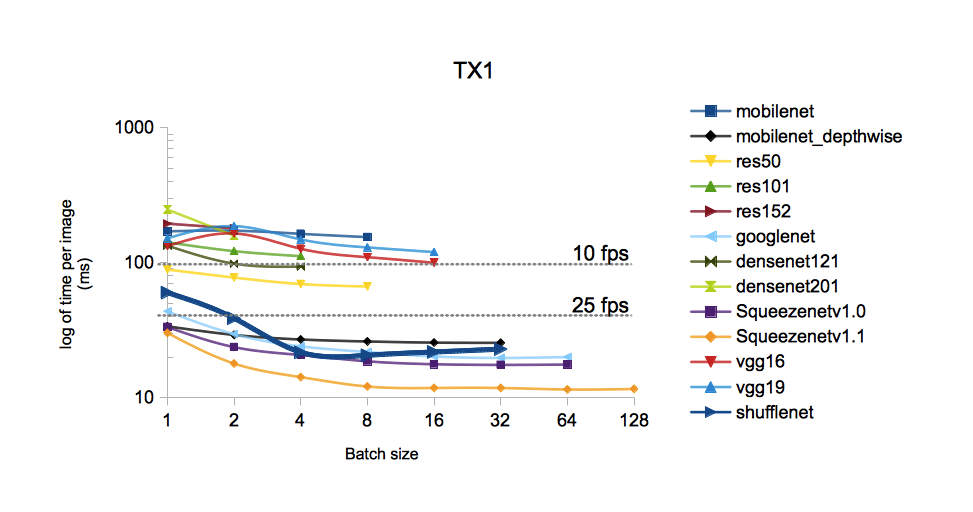
\includegraphics[width=.33\textwidth]{img/TX1_log.png}
    \caption{Comparativa entre Jetson TK1 (izquierda), Jetson Nano (centro) y Jetson TX1 (derecha). Escala logarítmica.}
    \label{fig:ben_nano_comp}
\end{figure}

\subsection{Google TPU \textit{Tensor Processing Unit}}

Google ha puesto a la venta su propio \textit{hardware} acelerador de cómputo, que hasta hace pocos meses no ofrecía. En su lugar, ofrecía servicios de computación en la nube como \textit{Google Colab}, en el que de forma gratuita se tiene acceso a un servidor para realizar cálculos en la nube con esta tecnología TPU que acelera en gran medida los tiempos de aprendizaje de las redes neuronales. La Figura \ref{fig:tpu} muestra una unidad de TPU de Google.

\begin{figure}[htp]
    \centering
    \captionsetup{justification=centering}
    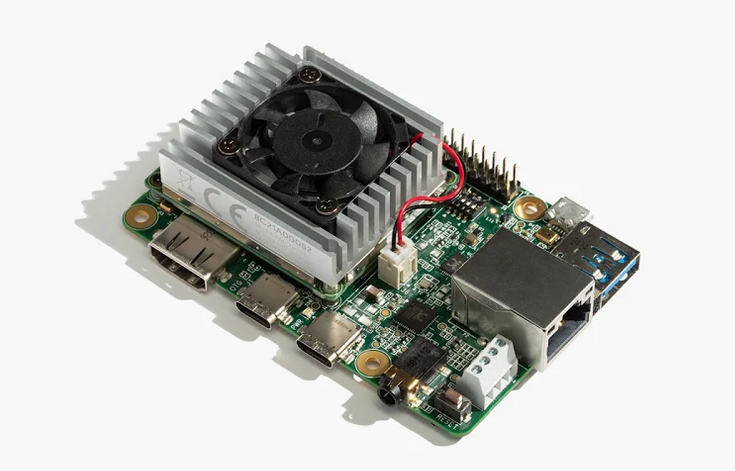
\includegraphics[width=.5\textwidth]{img/tpu.PNG}\hfill
    \caption{TPU de Google.}
    \label{fig:tpu}
\end{figure}

En 2018, Google presentó su propio \textit{hardware} acelerador de cómputo especializado en cálculo matricial y al que denominó TPU \cite{tpu}. Estas siglas, similares a las de GPU (\textit{Graphic Porcessing Unit}), vienen de \textit{Tensor Processing Unit} o Unidad de procesamiento de tensores. Un tensor no es más que una matriz multidimensional. La ventaja de las TPU es que pueden realizar cálculos en paralelo a una gran velocidad y, dado su carácter optimizado para el cálculo matricial (álgebra lineal), son ideales para la ejecución algoritmos de aprendizaje automático para visión artificial al ser la información que procesan estas redes matrices (imágenes).

No obstante, esta tecnología está pensada para ser utilizada en determinados ámbitos de trabajo concretos, de tal forma que en cómputo de carácter más general es más recomendable utilizar CPU o GPU.

\begin{itemize}
    \item CPU. Recomendado para realizar prototipos rápidos que requieran mucha flexibilidad. Entrenar modelos sencillos, pequeños y limitados.
    \item GPU. Modelos con un número notable de operaciones y con tamaños de lote grandes.
    \item TPU. Modelos de cómputo de matrices, con amplio tiempo de entrenamiento. Modelos muy grandes.
\end{itemize}

\begin{comment}
\section{Conclusiones}

Se han visto las tecnologías más punteras en cuanto a procesamiento de datos con redes neuronales, utilizando conjuntos de datos obtenidos para resolver el problema de la conducción autónoma. Además, se han visto las últimas tendencias en cuanto a \textit{hardware} acelerador de cómputo, con propuestas de diferentes empresas privadas que están a la cabeza en el sector tecnológico. Los algoritmos que se han explicado aquí son casos de éxito de los mismos en problemas de conducción autónoma, por lo que este TFM propone la ejecución de estos algoritmos en sistemas empotrados muy eficientes, de forma que se solvente el problema de cómputo de las redes neuronales, que necesitan hardware muy potente, y, por ende, muchos recursos en cuanto a alimentación de ese \textit{hardware} y espacio físico.

Las tecnologías explicadas en este estado del arte, intentarán aplicarse en este proyecto en mayor o menor medida, en cuanto a las capacidades y disponibilidad de \textit{hardware} en el momento de su desarrollo.
\end{comment}